\documentclass[1p]{elsarticle_modified}
%\bibliographystyle{elsarticle-num}

%\usepackage[colorlinks]{hyperref}
%\usepackage{abbrmath_seonhwa} %\Abb, \Ascr, \Acal ,\Abf, \Afrak
\usepackage{amsfonts}
\usepackage{amssymb}
\usepackage{amsmath}
\usepackage{amsthm}
\usepackage{scalefnt}
\usepackage{amsbsy}
\usepackage{kotex}
\usepackage{caption}
\usepackage{subfig}
\usepackage{color}
\usepackage{graphicx}
\usepackage{xcolor} %% white, black, red, green, blue, cyan, magenta, yellow
\usepackage{float}
\usepackage{setspace}
\usepackage{hyperref}

\usepackage{tikz}
\usetikzlibrary{arrows}

\usepackage{multirow}
\usepackage{array} % fixed length table
\usepackage{hhline}

%%%%%%%%%%%%%%%%%%%%%
\makeatletter
\renewcommand*\env@matrix[1][\arraystretch]{%
	\edef\arraystretch{#1}%
	\hskip -\arraycolsep
	\let\@ifnextchar\new@ifnextchar
	\array{*\c@MaxMatrixCols c}}
\makeatother %https://tex.stackexchange.com/questions/14071/how-can-i-increase-the-line-spacing-in-a-matrix
%%%%%%%%%%%%%%%

\usepackage[normalem]{ulem}

\newcommand{\msout}[1]{\ifmmode\text{\sout{\ensuremath{#1}}}\else\sout{#1}\fi}
%SOURCE: \msout is \stkout macro in https://tex.stackexchange.com/questions/20609/strikeout-in-math-mode

\newcommand{\cancel}[1]{
	\ifmmode
	{\color{red}\msout{#1}}
	\else
	{\color{red}\sout{#1}}
	\fi
}

\newcommand{\add}[1]{
	{\color{blue}\uwave{#1}}
}

\newcommand{\replace}[2]{
	\ifmmode
	{\color{red}\msout{#1}}{\color{blue}\uwave{#2}}
	\else
	{\color{red}\sout{#1}}{\color{blue}\uwave{#2}}
	\fi
}

\newcommand{\Sol}{\mathcal{S}} %segment
\newcommand{\D}{D} %diagram
\newcommand{\A}{\mathcal{A}} %arc


%%%%%%%%%%%%%%%%%%%%%%%%%%%%%5 test

\def\sl{\operatorname{\textup{SL}}(2,\Cbb)}
\def\psl{\operatorname{\textup{PSL}}(2,\Cbb)}
\def\quan{\mkern 1mu \triangleright \mkern 1mu}

\theoremstyle{definition}
\newtheorem{thm}{Theorem}[section]
\newtheorem{prop}[thm]{Proposition}
\newtheorem{lem}[thm]{Lemma}
\newtheorem{ques}[thm]{Question}
\newtheorem{cor}[thm]{Corollary}
\newtheorem{defn}[thm]{Definition}
\newtheorem{exam}[thm]{Example}
\newtheorem{rmk}[thm]{Remark}
\newtheorem{alg}[thm]{Algorithm}

\newcommand{\I}{\sqrt{-1}}
\begin{document}

%\begin{frontmatter}
%
%\title{Boundary parabolic representations of knots up to 8 crossings}
%
%%% Group authors per affiliation:
%\author{Yunhi Cho} 
%\address{Department of Mathematics, University of Seoul, Seoul, Korea}
%\ead{yhcho@uos.ac.kr}
%
%
%\author{Seonhwa Kim} %\fnref{s_kim}}
%\address{Center for Geometry and Physics, Institute for Basic Science, Pohang, 37673, Korea}
%\ead{ryeona17@ibs.re.kr}
%
%\author{Hyuk Kim}
%\address{Department of Mathematical Sciences, Seoul National University, Seoul 08826, Korea}
%\ead{hyukkim@snu.ac.kr}
%
%\author{Seokbeom Yoon}
%\address{Department of Mathematical Sciences, Seoul National University, Seoul, 08826,  Korea}
%\ead{sbyoon15@snu.ac.kr}
%
%\begin{abstract}
%We find all boundary parabolic representation of knots up to 8 crossings.
%
%\end{abstract}
%\begin{keyword}
%    \MSC[2010] 57M25 
%\end{keyword}
%
%\end{frontmatter}

%\linenumbers
%\tableofcontents
%
\newcommand\colored[1]{\textcolor{white}{\rule[-0.35ex]{0.8em}{1.4ex}}\kern-0.8em\color{red} #1}%
%\newcommand\colored[1]{\textcolor{white}{ #1}\kern-2.17ex	\textcolor{white}{ #1}\kern-1.81ex	\textcolor{white}{ #1}\kern-2.15ex\color{red}#1	}

{\Large $\underline{12a_{0517}~(K12a_{0517})}$}

\setlength{\tabcolsep}{10pt}
\renewcommand{\arraystretch}{1.6}
\vspace{1cm}\begin{tabular}{m{100pt}>{\centering\arraybackslash}m{274pt}}
\multirow{5}{120pt}{
	\centering
	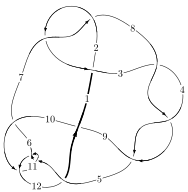
\includegraphics[width=112pt]{../../../GIT/diagram.site/Diagrams/png/1318_12a_0517.png}\\
\ \ \ A knot diagram\footnotemark}&
\allowdisplaybreaks
\textbf{Linearized knot diagam} \\
\cline{2-2}
 &
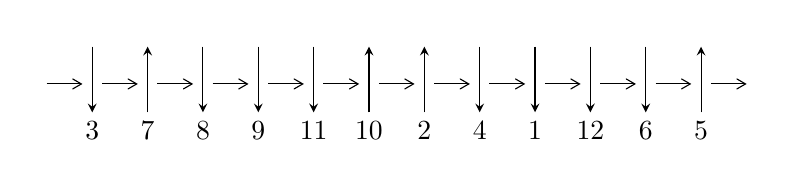
\begin{tikzpicture}[x=20pt, y=17pt]
	% nodes
	\node (C0) at (0, 0) {};
	\node (C1) at (1, 0) {};
	\node (C1U) at (1, +1) {};
	\node (C1D) at (1, -1) {3};

	\node (C2) at (2, 0) {};
	\node (C2U) at (2, +1) {};
	\node (C2D) at (2, -1) {7};

	\node (C3) at (3, 0) {};
	\node (C3U) at (3, +1) {};
	\node (C3D) at (3, -1) {8};

	\node (C4) at (4, 0) {};
	\node (C4U) at (4, +1) {};
	\node (C4D) at (4, -1) {9};

	\node (C5) at (5, 0) {};
	\node (C5U) at (5, +1) {};
	\node (C5D) at (5, -1) {11};

	\node (C6) at (6, 0) {};
	\node (C6U) at (6, +1) {};
	\node (C6D) at (6, -1) {10};

	\node (C7) at (7, 0) {};
	\node (C7U) at (7, +1) {};
	\node (C7D) at (7, -1) {2};

	\node (C8) at (8, 0) {};
	\node (C8U) at (8, +1) {};
	\node (C8D) at (8, -1) {4};

	\node (C9) at (9, 0) {};
	\node (C9U) at (9, +1) {};
	\node (C9D) at (9, -1) {1};

	\node (C10) at (10, 0) {};
	\node (C10U) at (10, +1) {};
	\node (C10D) at (10, -1) {12};

	\node (C11) at (11, 0) {};
	\node (C11U) at (11, +1) {};
	\node (C11D) at (11, -1) {6};

	\node (C12) at (12, 0) {};
	\node (C12U) at (12, +1) {};
	\node (C12D) at (12, -1) {5};
	\node (C13) at (13, 0) {};

	% arrows
	\draw[->,>={angle 60}]
	(C0) edge (C1) (C1) edge (C2) (C2) edge (C3) (C3) edge (C4) (C4) edge (C5) (C5) edge (C6) (C6) edge (C7) (C7) edge (C8) (C8) edge (C9) (C9) edge (C10) (C10) edge (C11) (C11) edge (C12) (C12) edge (C13) ;	\draw[->,>=stealth]
	(C1U) edge (C1D) (C2D) edge (C2U) (C3U) edge (C3D) (C4U) edge (C4D) (C5U) edge (C5D) (C6D) edge (C6U) (C7D) edge (C7U) (C8U) edge (C8D) (C9U) edge (C9D) (C10U) edge (C10D) (C11U) edge (C11D) (C12D) edge (C12U) ;
	\end{tikzpicture} \\
\hhline{~~} \\& 
\textbf{Solving Sequence} \\ \cline{2-2} 
 &
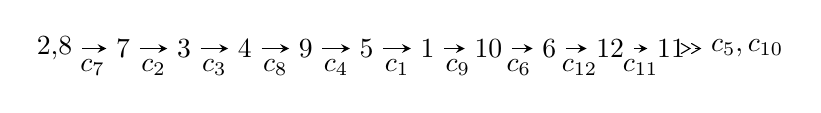
\begin{tikzpicture}[x=22pt, y=7pt]
	% node
	\node (A0) at (-1/8, 0) {2,8};
	\node (A1) at (1, 0) {7};
	\node (A2) at (2, 0) {3};
	\node (A3) at (3, 0) {4};
	\node (A4) at (4, 0) {9};
	\node (A5) at (5, 0) {5};
	\node (A6) at (6, 0) {1};
	\node (A7) at (7, 0) {10};
	\node (A8) at (8, 0) {6};
	\node (A9) at (9, 0) {12};
	\node (A10) at (10, 0) {11};
	\node (C1) at (1/2, -1) {$c_{7}$};
	\node (C2) at (3/2, -1) {$c_{2}$};
	\node (C3) at (5/2, -1) {$c_{3}$};
	\node (C4) at (7/2, -1) {$c_{8}$};
	\node (C5) at (9/2, -1) {$c_{4}$};
	\node (C6) at (11/2, -1) {$c_{1}$};
	\node (C7) at (13/2, -1) {$c_{9}$};
	\node (C8) at (15/2, -1) {$c_{6}$};
	\node (C9) at (17/2, -1) {$c_{12}$};
	\node (C10) at (19/2, -1) {$c_{11}$};
	\node (A11) at (45/4, 0) {$c_{5},c_{10}$};

	% edge
	\draw[->,>=stealth]	
	(A0) edge (A1) (A1) edge (A2) (A2) edge (A3) (A3) edge (A4) (A4) edge (A5) (A5) edge (A6) (A6) edge (A7) (A7) edge (A8) (A8) edge (A9) (A9) edge (A10) ;
	\draw[->>,>={angle 60}]	
	(A10) edge (A11);
\end{tikzpicture} \\ 

\end{tabular} \\

\footnotetext{
The image of knot diagram is generated by the software ``\textbf{Draw programme}" developed by Andrew Bartholomew(\url{http://www.layer8.co.uk/maths/draw/index.htm\#Running-draw}), where we modified some parts for our purpose(\url{https://github.com/CATsTAILs/LinksPainter}).
}\phantom \\ \newline 
\centering \textbf{Ideals for irreducible components\footnotemark of $X_{\text{par}}$} 
 
\begin{align*}
I^u_{1}&=\langle 
u^{72}- u^{71}+\cdots+2 u-1\rangle \\
\\
\end{align*}
\raggedright * 1 irreducible components of $\dim_{\mathbb{C}}=0$, with total 72 representations.\\
\footnotetext{All coefficients of polynomials are rational numbers. But the coefficients are sometimes approximated in decimal forms when there is not enough margin.}
\newpage
\renewcommand{\arraystretch}{1}
\centering \section*{I. $I^u_{1}= \langle u^{72}- u^{71}+\cdots+2 u-1 \rangle$}
\flushleft \textbf{(i) Arc colorings}\\
\begin{tabular}{m{7pt} m{180pt} m{7pt} m{180pt} }
\flushright $a_{2}=$&$\begin{pmatrix}0\\u\end{pmatrix}$ \\
\flushright $a_{8}=$&$\begin{pmatrix}1\\0\end{pmatrix}$ \\
\flushright $a_{7}=$&$\begin{pmatrix}1\\u^2\end{pmatrix}$ \\
\flushright $a_{3}=$&$\begin{pmatrix}u\\u^3+u\end{pmatrix}$ \\
\flushright $a_{4}=$&$\begin{pmatrix}- u^3\\u^3+u\end{pmatrix}$ \\
\flushright $a_{9}=$&$\begin{pmatrix}- u^6- u^4+1\\u^6+2 u^4+u^2\end{pmatrix}$ \\
\flushright $a_{5}=$&$\begin{pmatrix}u^9+2 u^7+u^5-2 u^3- u\\- u^9-3 u^7-3 u^5+u\end{pmatrix}$ \\
\flushright $a_{1}=$&$\begin{pmatrix}u^3\\u^5+u^3+u\end{pmatrix}$ \\
\flushright $a_{10}=$&$\begin{pmatrix}- u^{14}-3 u^{12}-4 u^{10}- u^8+1\\- u^{16}-4 u^{14}-8 u^{12}-8 u^{10}-4 u^8+2 u^6+4 u^4+2 u^2\end{pmatrix}$ \\
\flushright $a_{6}=$&$\begin{pmatrix}u^{28}+7 u^{26}+\cdots+u^2+1\\u^{30}+8 u^{28}+\cdots+2 u^4+u^2\end{pmatrix}$ \\
\flushright $a_{12}=$&$\begin{pmatrix}- u^{23}-6 u^{21}-16 u^{19}-20 u^{17}-4 u^{15}+22 u^{13}+26 u^{11}+6 u^9-9 u^7-6 u^5\\u^{23}+7 u^{21}+\cdots+2 u^3+u\end{pmatrix}$ \\
\flushright $a_{11}=$&$\begin{pmatrix}u^{62}+17 u^{60}+\cdots-6 u^6+1\\- u^{62}-18 u^{60}+\cdots+8 u^4+3 u^2\end{pmatrix}$\\&\end{tabular}
\flushleft \textbf{(ii) Obstruction class $= -1$}\\~\\
\flushleft \textbf{(iii) Cusp Shapes $= 4 u^{70}-4 u^{69}+\cdots+8 u-10$}\\~\\
\newpage\renewcommand{\arraystretch}{1}
\flushleft \textbf{(iv) u-Polynomials at the component}\newline \\
\begin{tabular}{m{50pt}|m{274pt}}
Crossings & \hspace{64pt}u-Polynomials at each crossing \\
\hline $$\begin{aligned}c_{1}\end{aligned}$$&$\begin{aligned}
&u^{72}+41 u^{71}+\cdots-10 u^2+1
\end{aligned}$\\
\hline $$\begin{aligned}c_{2},c_{7}\end{aligned}$$&$\begin{aligned}
&u^{72}+u^{71}+\cdots-2 u-1
\end{aligned}$\\
\hline $$\begin{aligned}c_{3},c_{4},c_{8}\end{aligned}$$&$\begin{aligned}
&u^{72}- u^{71}+\cdots+42 u-17
\end{aligned}$\\
\hline $$\begin{aligned}c_{5},c_{11}\end{aligned}$$&$\begin{aligned}
&u^{72}- u^{71}+\cdots+2 u^3-1
\end{aligned}$\\
\hline $$\begin{aligned}c_{6},c_{12}\end{aligned}$$&$\begin{aligned}
&u^{72}-3 u^{71}+\cdots-18 u+3
\end{aligned}$\\
\hline $$\begin{aligned}c_{9}\end{aligned}$$&$\begin{aligned}
&u^{72}-11 u^{71}+\cdots-18764 u+1889
\end{aligned}$\\
\hline $$\begin{aligned}c_{10}\end{aligned}$$&$\begin{aligned}
&u^{72}+39 u^{71}+\cdots-2 u^2+1
\end{aligned}$\\
\hline
\end{tabular}\\~\\
\newpage\renewcommand{\arraystretch}{1}
\flushleft \textbf{(v) Riley Polynomials at the component}\newline \\
\begin{tabular}{m{50pt}|m{274pt}}
Crossings & \hspace{64pt}Riley Polynomials at each crossing \\
\hline $$\begin{aligned}c_{1}\end{aligned}$$&$\begin{aligned}
&y^{72}-19 y^{71}+\cdots-20 y+1
\end{aligned}$\\
\hline $$\begin{aligned}c_{2},c_{7}\end{aligned}$$&$\begin{aligned}
&y^{72}+41 y^{71}+\cdots-10 y^2+1
\end{aligned}$\\
\hline $$\begin{aligned}c_{3},c_{4},c_{8}\end{aligned}$$&$\begin{aligned}
&y^{72}-79 y^{71}+\cdots-10740 y+289
\end{aligned}$\\
\hline $$\begin{aligned}c_{5},c_{11}\end{aligned}$$&$\begin{aligned}
&y^{72}-39 y^{71}+\cdots-2 y^2+1
\end{aligned}$\\
\hline $$\begin{aligned}c_{6},c_{12}\end{aligned}$$&$\begin{aligned}
&y^{72}+61 y^{71}+\cdots-624 y+9
\end{aligned}$\\
\hline $$\begin{aligned}c_{9}\end{aligned}$$&$\begin{aligned}
&y^{72}-31 y^{71}+\cdots-2222228 y+3568321
\end{aligned}$\\
\hline $$\begin{aligned}c_{10}\end{aligned}$$&$\begin{aligned}
&y^{72}-11 y^{71}+\cdots-4 y+1
\end{aligned}$\\
\hline
\end{tabular}\\~\\
\newpage\flushleft \textbf{(vi) Complex Volumes and Cusp Shapes}
$$\begin{array}{c|c|c}  
\text{Solutions to }I^u_{1}& \I (\text{vol} + \sqrt{-1}CS) & \text{Cusp shape}\\
 \hline 
\begin{aligned}
u &= -0.439849 + 0.927313 I\end{aligned}
 & \phantom{-}0.59296 - 2.15388 I & \phantom{-0.000000 -}0. + 3.34635 I \\ \hline\begin{aligned}
u &= -0.439849 - 0.927313 I\end{aligned}
 & \phantom{-}0.59296 + 2.15388 I & \phantom{-0.000000 } 0. - 3.34635 I \\ \hline\begin{aligned}
u &= \phantom{-}0.127748 + 0.947194 I\end{aligned}
 & -2.02452 - 1.35976 I & -10.77685 + 3.46053 I \\ \hline\begin{aligned}
u &= \phantom{-}0.127748 - 0.947194 I\end{aligned}
 & -2.02452 + 1.35976 I & -10.77685 - 3.46053 I \\ \hline\begin{aligned}
u &= -0.351185 + 0.866043 I\end{aligned}
 & -0.38120 - 1.62589 I & -2.66925 + 4.11942 I \\ \hline\begin{aligned}
u &= -0.351185 - 0.866043 I\end{aligned}
 & -0.38120 + 1.62589 I & -2.66925 - 4.11942 I \\ \hline\begin{aligned}
u &= \phantom{-}0.461087 + 0.962460 I\end{aligned}
 & \phantom{-}0.08467 + 6.28501 I & \phantom{-0.000000 } 0 \\ \hline\begin{aligned}
u &= \phantom{-}0.461087 - 0.962460 I\end{aligned}
 & \phantom{-}0.08467 - 6.28501 I & \phantom{-0.000000 } 0 \\ \hline\begin{aligned}
u &= \phantom{-}0.344819 + 1.019280 I\end{aligned}
 & -3.62015 + 2.92141 I & \phantom{-0.000000 } 0 \\ \hline\begin{aligned}
u &= \phantom{-}0.344819 - 1.019280 I\end{aligned}
 & -3.62015 - 2.92141 I & \phantom{-0.000000 } 0 \\ \hline\begin{aligned}
u &= \phantom{-}0.206282 + 1.082360 I\end{aligned}
 & -4.82312 - 0.17742 I & \phantom{-0.000000 } 0 \\ \hline\begin{aligned}
u &= \phantom{-}0.206282 - 1.082360 I\end{aligned}
 & -4.82312 + 0.17742 I & \phantom{-0.000000 } 0 \\ \hline\begin{aligned}
u &= \phantom{-}0.456210 + 0.765907 I\end{aligned}
 & -3.17229 - 2.09595 I & -5.70344 - 0.42832 I \\ \hline\begin{aligned}
u &= \phantom{-}0.456210 - 0.765907 I\end{aligned}
 & -3.17229 + 2.09595 I & -5.70344 + 0.42832 I \\ \hline\begin{aligned}
u &= -0.189472 + 1.099100 I\end{aligned}
 & -8.15714 + 4.74025 I & \phantom{-0.000000 } 0 \\ \hline\begin{aligned}
u &= -0.189472 - 1.099100 I\end{aligned}
 & -8.15714 - 4.74025 I & \phantom{-0.000000 } 0 \\ \hline\begin{aligned}
u &= \phantom{-}0.882022 + 0.044279 I\end{aligned}
 & -11.98020 - 0.80891 I & -10.79930 - 0.35413 I \\ \hline\begin{aligned}
u &= \phantom{-}0.882022 - 0.044279 I\end{aligned}
 & -11.98020 + 0.80891 I & -10.79930 + 0.35413 I \\ \hline\begin{aligned}
u &= \phantom{-}0.879727 + 0.056445 I\end{aligned}
 & -11.1703 - 9.8634 I & -9.53343 + 5.93137 I \\ \hline\begin{aligned}
u &= \phantom{-}0.879727 - 0.056445 I\end{aligned}
 & -11.1703 + 9.8634 I & -9.53343 - 5.93137 I \\ \hline\begin{aligned}
u &= -0.875707 + 0.050791 I\end{aligned}
 & -7.91972 + 4.99528 I & -6.55693 - 2.82964 I \\ \hline\begin{aligned}
u &= -0.875707 - 0.050791 I\end{aligned}
 & -7.91972 - 4.99528 I & -6.55693 + 2.82964 I \\ \hline\begin{aligned}
u &= -0.225561 + 1.101690 I\end{aligned}
 & -8.49214 - 4.06217 I & \phantom{-0.000000 } 0 \\ \hline\begin{aligned}
u &= -0.225561 - 1.101690 I\end{aligned}
 & -8.49214 + 4.06217 I & \phantom{-0.000000 } 0 \\ \hline\begin{aligned}
u &= \phantom{-}0.474807 + 1.020050 I\end{aligned}
 & -2.88869 + 6.40679 I & \phantom{-0.000000 } 0 \\ \hline\begin{aligned}
u &= \phantom{-}0.474807 - 1.020050 I\end{aligned}
 & -2.88869 - 6.40679 I & \phantom{-0.000000 } 0 \\ \hline\begin{aligned}
u &= -0.489288 + 1.023920 I\end{aligned}
 & -5.98929 - 11.10170 I & \phantom{-0.000000 } 0 \\ \hline\begin{aligned}
u &= -0.489288 - 1.023920 I\end{aligned}
 & -5.98929 + 11.10170 I & \phantom{-0.000000 } 0 \\ \hline\begin{aligned}
u &= -0.862003\phantom{ +0.000000I}\end{aligned}
 & -7.62273\phantom{ +0.000000I} & -11.5620\phantom{ +0.000000I} \\ \hline\begin{aligned}
u &= -0.467805 + 1.041330 I\end{aligned}
 & -6.73822 - 2.46906 I & \phantom{-0.000000 } 0\\
 \hline 
 \end{array}$$\newpage$$\begin{array}{c|c|c}  
\text{Solutions to }I^u_{1}& \I (\text{vol} + \sqrt{-1}CS) & \text{Cusp shape}\\
 \hline 
\begin{aligned}
u &= -0.467805 - 1.041330 I\end{aligned}
 & -6.73822 + 2.46906 I & \phantom{-0.000000 } 0 \\ \hline\begin{aligned}
u &= -0.838828 + 0.044532 I\end{aligned}
 & -3.98379 + 5.00843 I & -5.49188 - 6.00077 I \\ \hline\begin{aligned}
u &= -0.838828 - 0.044532 I\end{aligned}
 & -3.98379 - 5.00843 I & -5.49188 + 6.00077 I \\ \hline\begin{aligned}
u &= \phantom{-}0.474990 + 0.690912 I\end{aligned}
 & -2.96171 + 6.03372 I & -4.87395 - 7.35313 I \\ \hline\begin{aligned}
u &= \phantom{-}0.474990 - 0.690912 I\end{aligned}
 & -2.96171 - 6.03372 I & -4.87395 + 7.35313 I \\ \hline\begin{aligned}
u &= \phantom{-}0.825126 + 0.022311 I\end{aligned}
 & -2.88998 - 0.66859 I & -2.98851 - 0.14329 I \\ \hline\begin{aligned}
u &= \phantom{-}0.825126 - 0.022311 I\end{aligned}
 & -2.88998 + 0.66859 I & -2.98851 + 0.14329 I \\ \hline\begin{aligned}
u &= -0.413409 + 0.683683 I\end{aligned}
 & \phantom{-}0.00742 - 1.75216 I & -1.16689 + 4.43589 I \\ \hline\begin{aligned}
u &= -0.413409 - 0.683683 I\end{aligned}
 & \phantom{-}0.00742 + 1.75216 I & -1.16689 - 4.43589 I \\ \hline\begin{aligned}
u &= \phantom{-}0.450918 + 1.227690 I\end{aligned}
 & -6.60070 + 3.85865 I & \phantom{-0.000000 } 0 \\ \hline\begin{aligned}
u &= \phantom{-}0.450918 - 1.227690 I\end{aligned}
 & -6.60070 - 3.85865 I & \phantom{-0.000000 } 0 \\ \hline\begin{aligned}
u &= -0.438765 + 1.234300 I\end{aligned}
 & -7.81587 + 0.51539 I & \phantom{-0.000000 } 0 \\ \hline\begin{aligned}
u &= -0.438765 - 1.234300 I\end{aligned}
 & -7.81587 - 0.51539 I & \phantom{-0.000000 } 0 \\ \hline\begin{aligned}
u &= \phantom{-}0.470711 + 1.225250 I\end{aligned}
 & -6.45782 + 5.32632 I & \phantom{-0.000000 } 0 \\ \hline\begin{aligned}
u &= \phantom{-}0.470711 - 1.225250 I\end{aligned}
 & -6.45782 - 5.32632 I & \phantom{-0.000000 } 0 \\ \hline\begin{aligned}
u &= -0.442364 + 0.520924 I\end{aligned}
 & \phantom{-}1.71123 - 1.63055 I & \phantom{-}1.63060 + 4.27651 I \\ \hline\begin{aligned}
u &= -0.442364 - 0.520924 I\end{aligned}
 & \phantom{-}1.71123 + 1.63055 I & \phantom{-}1.63060 - 4.27651 I \\ \hline\begin{aligned}
u &= -0.481138 + 1.227880 I\end{aligned}
 & -7.51183 - 9.76537 I & \phantom{-0.000000 } 0 \\ \hline\begin{aligned}
u &= -0.481138 - 1.227880 I\end{aligned}
 & -7.51183 + 9.76537 I & \phantom{-0.000000 } 0 \\ \hline\begin{aligned}
u &= -0.590261 + 0.336282 I\end{aligned}
 & -4.08423 + 6.85269 I & -6.08983 - 5.98107 I \\ \hline\begin{aligned}
u &= -0.590261 - 0.336282 I\end{aligned}
 & -4.08423 - 6.85269 I & -6.08983 + 5.98107 I \\ \hline\begin{aligned}
u &= -0.463776 + 1.244240 I\end{aligned}
 & -11.37070 - 4.72051 I & \phantom{-0.000000 } 0 \\ \hline\begin{aligned}
u &= -0.463776 - 1.244240 I\end{aligned}
 & -11.37070 + 4.72051 I & \phantom{-0.000000 } 0 \\ \hline\begin{aligned}
u &= -0.436607 + 1.257510 I\end{aligned}
 & -11.90830 + 0.38192 I & \phantom{-0.000000 } 0 \\ \hline\begin{aligned}
u &= -0.436607 - 1.257510 I\end{aligned}
 & -11.90830 - 0.38192 I & \phantom{-0.000000 } 0 \\ \hline\begin{aligned}
u &= \phantom{-}0.433445 + 1.260510 I\end{aligned}
 & -15.1956 - 5.2532 I & \phantom{-0.000000 } 0 \\ \hline\begin{aligned}
u &= \phantom{-}0.433445 - 1.260510 I\end{aligned}
 & -15.1956 + 5.2532 I & \phantom{-0.000000 } 0 \\ \hline\begin{aligned}
u &= \phantom{-}0.441141 + 1.260650 I\end{aligned}
 & -15.9636 + 3.8514 I & \phantom{-0.000000 } 0 \\ \hline\begin{aligned}
u &= \phantom{-}0.441141 - 1.260650 I\end{aligned}
 & -15.9636 - 3.8514 I & \phantom{-0.000000 } 0 \\ \hline\begin{aligned}
u &= -0.490825 + 1.242560 I\end{aligned}
 & -11.5116 - 9.9029 I & \phantom{-0.000000 } 0\\
 \hline 
 \end{array}$$\newpage$$\begin{array}{c|c|c}  
\text{Solutions to }I^u_{1}& \I (\text{vol} + \sqrt{-1}CS) & \text{Cusp shape}\\
 \hline 
\begin{aligned}
u &= -0.490825 - 1.242560 I\end{aligned}
 & -11.5116 + 9.9029 I & \phantom{-0.000000 } 0 \\ \hline\begin{aligned}
u &= \phantom{-}0.494249 + 1.243290 I\end{aligned}
 & -14.7502 + 14.8001 I & \phantom{-0.000000 } 0 \\ \hline\begin{aligned}
u &= \phantom{-}0.494249 - 1.243290 I\end{aligned}
 & -14.7502 - 14.8001 I & \phantom{-0.000000 } 0 \\ \hline\begin{aligned}
u &= \phantom{-}0.488923 + 1.246820 I\end{aligned}
 & -15.6129 + 5.7245 I & \phantom{-0.000000 } 0 \\ \hline\begin{aligned}
u &= \phantom{-}0.488923 - 1.246820 I\end{aligned}
 & -15.6129 - 5.7245 I & \phantom{-0.000000 } 0 \\ \hline\begin{aligned}
u &= \phantom{-}0.477316 + 0.439878 I\end{aligned}
 & \phantom{-}1.50816 - 2.35510 I & \phantom{-}0.54892 + 4.70586 I \\ \hline\begin{aligned}
u &= \phantom{-}0.477316 - 0.439878 I\end{aligned}
 & \phantom{-}1.50816 + 2.35510 I & \phantom{-}0.54892 - 4.70586 I \\ \hline\begin{aligned}
u &= -0.586128 + 0.275072 I\end{aligned}
 & -4.62644 - 1.65735 I & -7.50243 + 0.63837 I \\ \hline\begin{aligned}
u &= -0.586128 - 0.275072 I\end{aligned}
 & -4.62644 + 1.65735 I & -7.50243 - 0.63837 I \\ \hline\begin{aligned}
u &= \phantom{-}0.556736 + 0.320665 I\end{aligned}
 & -0.97920 - 2.29313 I & -2.83779 + 3.07654 I \\ \hline\begin{aligned}
u &= \phantom{-}0.556736 - 0.320665 I\end{aligned}
 & -0.97920 + 2.29313 I & -2.83779 - 3.07654 I \\ \hline\begin{aligned}
u &= \phantom{-}0.411425\phantom{ +0.000000I}\end{aligned}
 & -1.15550\phantom{ +0.000000I} & -8.76440\phantom{ +0.000000I}\\
 \hline 
 \end{array}$$\newpage
\newpage\renewcommand{\arraystretch}{1}
\centering \section*{ II. u-Polynomials}
\begin{tabular}{m{50pt}|m{274pt}}
Crossings & \hspace{64pt}u-Polynomials at each crossing \\
\hline $$\begin{aligned}c_{1}\end{aligned}$$&$\begin{aligned}
&u^{72}+41 u^{71}+\cdots-10 u^2+1
\end{aligned}$\\
\hline $$\begin{aligned}c_{2},c_{7}\end{aligned}$$&$\begin{aligned}
&u^{72}+u^{71}+\cdots-2 u-1
\end{aligned}$\\
\hline $$\begin{aligned}c_{3},c_{4},c_{8}\end{aligned}$$&$\begin{aligned}
&u^{72}- u^{71}+\cdots+42 u-17
\end{aligned}$\\
\hline $$\begin{aligned}c_{5},c_{11}\end{aligned}$$&$\begin{aligned}
&u^{72}- u^{71}+\cdots+2 u^3-1
\end{aligned}$\\
\hline $$\begin{aligned}c_{6},c_{12}\end{aligned}$$&$\begin{aligned}
&u^{72}-3 u^{71}+\cdots-18 u+3
\end{aligned}$\\
\hline $$\begin{aligned}c_{9}\end{aligned}$$&$\begin{aligned}
&u^{72}-11 u^{71}+\cdots-18764 u+1889
\end{aligned}$\\
\hline $$\begin{aligned}c_{10}\end{aligned}$$&$\begin{aligned}
&u^{72}+39 u^{71}+\cdots-2 u^2+1
\end{aligned}$\\
\hline
\end{tabular}\newpage\renewcommand{\arraystretch}{1}
\centering \section*{ III. Riley Polynomials}
\begin{tabular}{m{50pt}|m{274pt}}
Crossings & \hspace{64pt}Riley Polynomials at each crossing \\
\hline $$\begin{aligned}c_{1}\end{aligned}$$&$\begin{aligned}
&y^{72}-19 y^{71}+\cdots-20 y+1
\end{aligned}$\\
\hline $$\begin{aligned}c_{2},c_{7}\end{aligned}$$&$\begin{aligned}
&y^{72}+41 y^{71}+\cdots-10 y^2+1
\end{aligned}$\\
\hline $$\begin{aligned}c_{3},c_{4},c_{8}\end{aligned}$$&$\begin{aligned}
&y^{72}-79 y^{71}+\cdots-10740 y+289
\end{aligned}$\\
\hline $$\begin{aligned}c_{5},c_{11}\end{aligned}$$&$\begin{aligned}
&y^{72}-39 y^{71}+\cdots-2 y^2+1
\end{aligned}$\\
\hline $$\begin{aligned}c_{6},c_{12}\end{aligned}$$&$\begin{aligned}
&y^{72}+61 y^{71}+\cdots-624 y+9
\end{aligned}$\\
\hline $$\begin{aligned}c_{9}\end{aligned}$$&$\begin{aligned}
&y^{72}-31 y^{71}+\cdots-2222228 y+3568321
\end{aligned}$\\
\hline $$\begin{aligned}c_{10}\end{aligned}$$&$\begin{aligned}
&y^{72}-11 y^{71}+\cdots-4 y+1
\end{aligned}$\\
\hline
\end{tabular}
\vskip 2pc
\end{document}